\section{Data}
\label{sec:data}

The dataset used in this study is made by around 1700 overlapping aerial images taken by drones at Texas A\&M AgriLife Research\'s Brazos Bottom Farm in Burleson County, Texas (headquarters at 30.549635N, 96.436821W) \cite{shi_2021_5089956}.

UAVs were operated by three separate flight teams and were equipped with several sensors, auto-pilot and stabilization systems.
Most flights were made within 2.0h of solar noon. Flight and sensor parameters were configured to ensure collection of high-quality images with adequate overlap between images for mosaicking purposes, and to minimize pixel smearing.
For this case study the images were taken with a X88 octocopter UAV at a typical flying altitude of 15-20m, with a DJIP3-005 4K Camera and a resolution of 4000x3000 pixels.

Approximate locations of raw images (longitude, latitude, and altitude) were recorded by an onboard GPS, however, its accuracy is not high enough for direct georeferencing. Eight Ground Control Points (GCPs) were installed around the study area for accurate geo-referencing, geo-correction, and co-registration of UAS data.

\subsection{Preprocessing}
\label{sec:preprocessing}

Significant long-term challenges related to data collection/processing and interpretation of the processed data need to be addressed before breeders can fully embrace these systems. As raw data moves through the application development pipeline [\ref{fig:dev_pipeline}].
\begin{figure}[h!]
    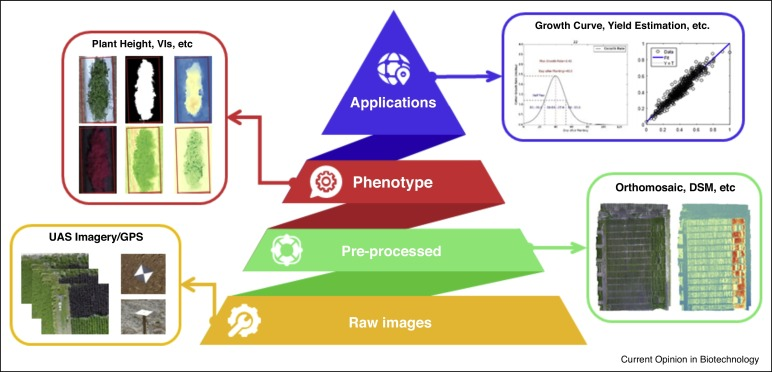
\includegraphics[width=\linewidth]{../images/dev_pipeline} 
    \caption{UAVs application development workflow. Figure from \cite{jung2021potential}.}
    \label{fig:dev_pipeline}
\end{figure}

No further post-processing has been applied to the images as it have been performed by the authors of the dataset.

Because of the time between the ground truth measurement and the generation of the DSM for height estimation, the ground truth values were averaged between the two.

GCPs are critical for georeferencing the images and therefore for the generation of the orthomosaic. The $61x61cm$ concrete tiles were installed at the corners and interior locations of all UAVs\' routes and were painted black, dark gray and light gray ($\approx$ 10\%, 20\% and 40\% reflectance).

The GCPs coordinates were converted from the 

The GCPs coordinates have been used with the GCPEditorPro software to identify the tiles on the ground within the overlaying images collected by the UAVs.
This lead to the georeferencing of the images that was supplied to the WebODM software to generate an orthomosaic of the field [\ref{fig:orthomosaic}].

Finally, the plots were extracted with the Python Shapefile Library \footnote{PyShp reads and writes ESRI Shapefiles in pure Python: \url{https://github.com/GeospatialPython/pyshp}} from the orthomosaic by using the shapefile provided in the dataset and then matched to the ground truth records to assign an height value to each of them.

\begin{figure}[b!]
    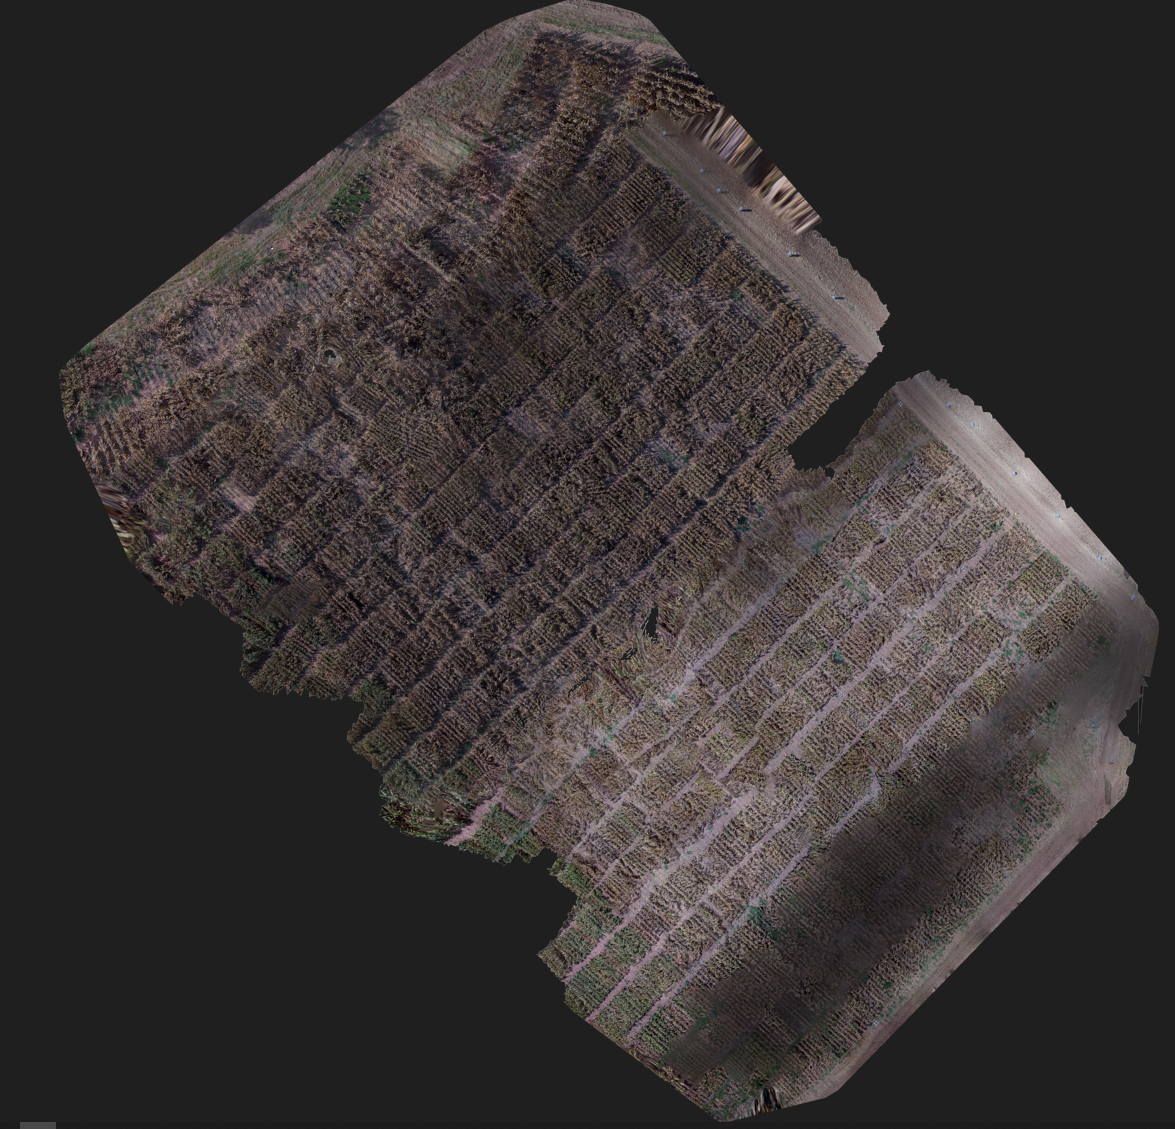
\includegraphics[width=\linewidth]{../images/orthomosaic} 
    \caption{Orthomosaic of the agricultural field. Produced with WebODM.}
    \label{fig:orthomosaic}
\end{figure}